\title{Lab and Machine Setup}
\author{
    Author: Yusef Karim \\
    Instructor: Jacques Béland \\
    Department of Computing \& Information Systems \\
}
\date{\today}

\documentclass[12pt]{article}
\usepackage[a4paper,margin=1in,footskip=0.25in]{geometry}
\usepackage{hyperref}
\usepackage{graphicx}
\usepackage{float}

\begin{document}
\maketitle


\section{Purpose}
In this lab we will be configuring two different test environments. The first will be a Linux virtual machine which will allow for testing of x86 exploits, the second will be a physical computer (Raspberry Pi) which allow for testing of ARM based exploits.
\paragraph{Note:}
Specifics will be left out, such as how to use Virtualbox to create virtual machines, how to install Linux, and some post-installation setup. What {\bfseries will} be shown and explained is the all relevant processes used to create a suitable test environemnt (with brief descriptions to why they are useful) and the end product.


\section{Ubuntu Virtual Machine}\label{ubuntu}
Virtualbox was used to create a 32-bit Ubuntu Server 16.04.5 virtual machine (get it \href{https://www.ubuntu.com/download/alternative-downloads}{here}), all that had to be done was use the Ubuntu ISO image then follow the GUI based installer to setup the machine in Virtualbox.

\begin{figure}[H]
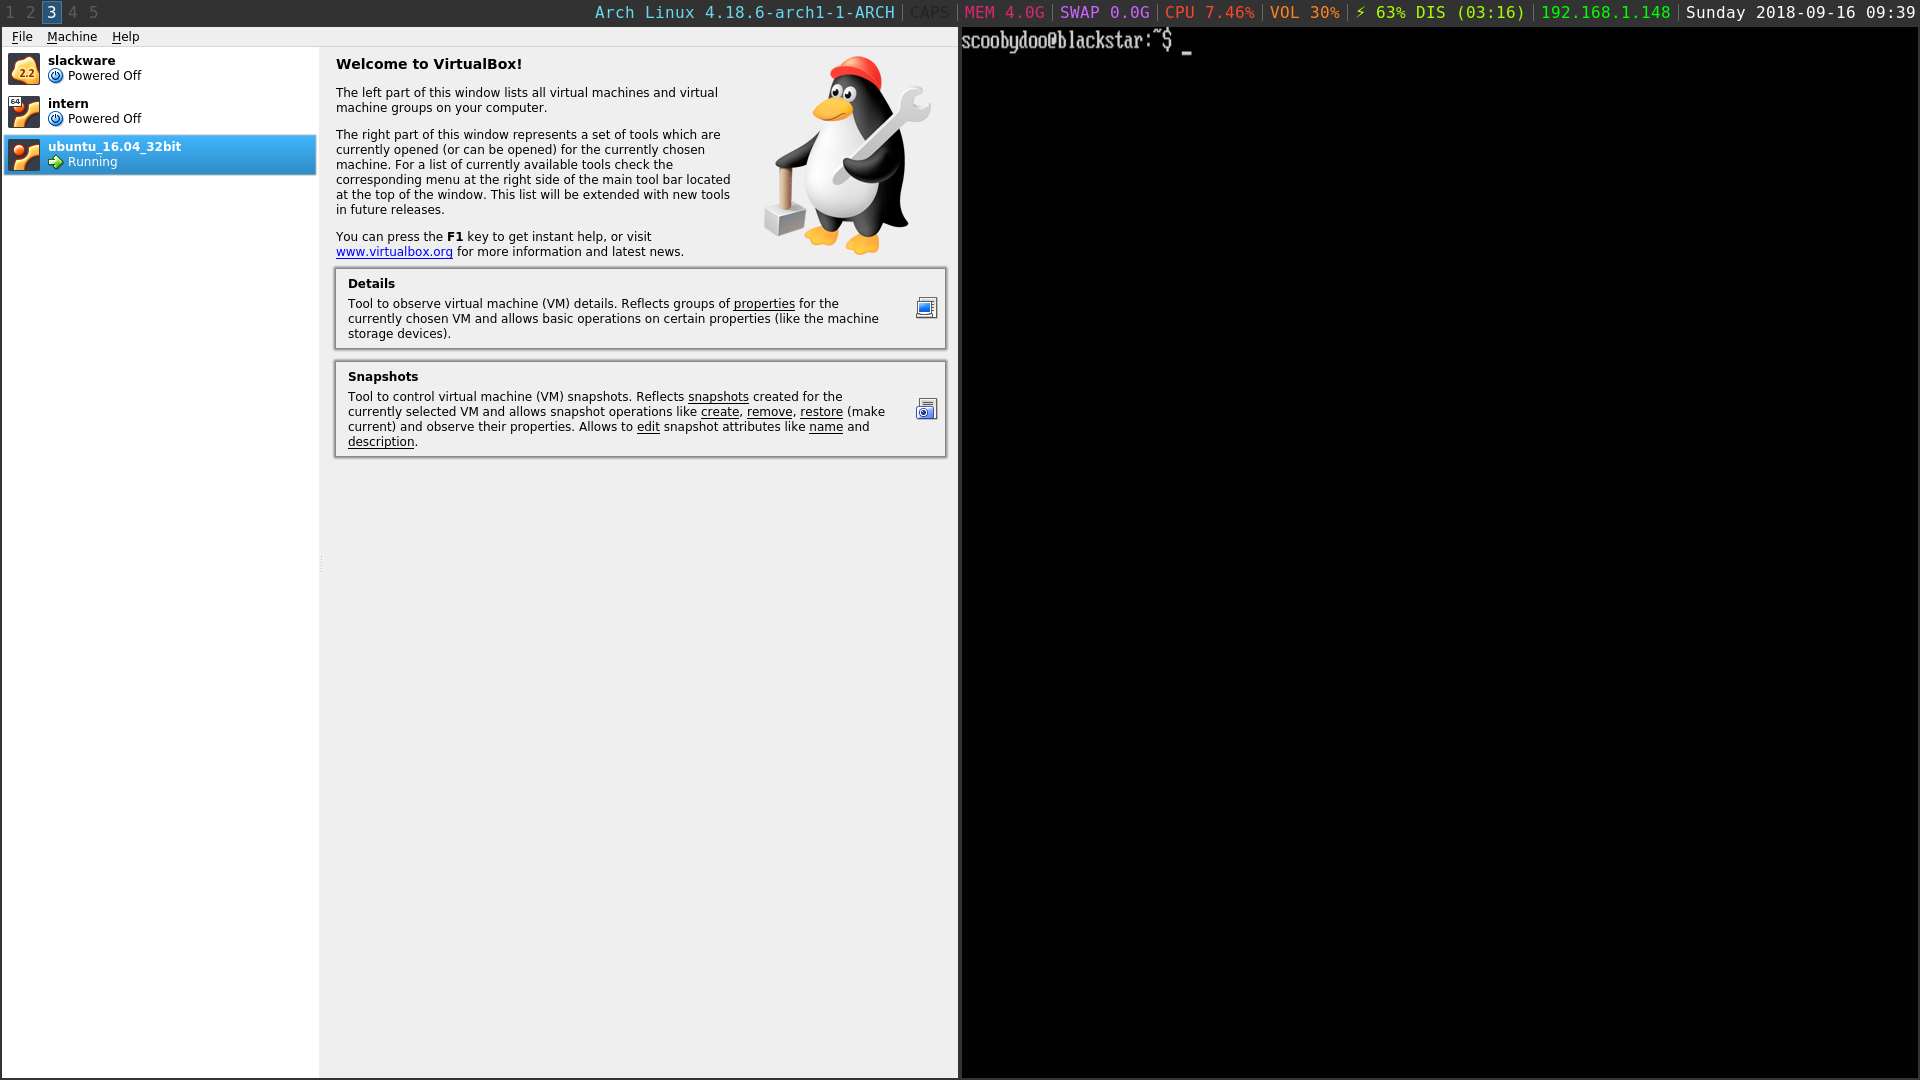
\includegraphics[width=15cm, height=8cm]{virtualbox_ubuntu.png}
\caption{Ubuntu 16.04 virtual machine running in Virtualbox after setup}
\end{figure}

This version of Ubuntu uses Linux kernel version 4.4.0 which has several security features to help prevent exploiting. The main security feature is Address Space Layout Randomization (ASLR) which is used to randomize memory (stack is the primary concern) everytime a program is executed. To disable this we can use sysctl, which in turn edits the value in the file /proc/sys/kernel/randomize\_va\_space.
\begin{verbatim}
sudo su
sysctl kernel.randomize_va_space=0
\end{verbatim}
Running this command, will disable ASLR but the changes will no be kept after rebooting, for this we can make a file in /etc/sysctl.d/ that will set this kernel parameter on bootup.
\begin{verbatim}
cd /etc/sysctl.d/
vim 1-aslr.conf
ADD THIS -> kernel.randomize_va_space = 0
reboot
sysctl kernel.randomize_va_space
OUTPUT -> kernel.randomize_va_space = 0
\end{verbatim}

Now that kernel security features have been dealt with, we can now start looking at what features the compiler implements for security. Currently Ubuntu 16.04 is using GCC version 5.4.0, which has several security features when compiling a C program. These features help prevent buffer overflows (via a stack protector), and prevent arbitrary commands being executed from within the stack. This means to compile a program we should use the following command:

\begin{verbatim}
gcc -fno-stack-protector -mpreferred-stack-boundary=2 -z execstack -ggdb
<YOUR CODE.c> -o <YOUR VULNERABLE EXECUTABLE>
\end{verbatim}

One last thing that will prove useful in the future is changing the ulimit to allow core files to be dumped when a program error occurs. This is done by running the following command:
\begin{verbatim}
ulimit -c unlimited
\end{verbatim}

To test our environment a short and potentially vulnerable program was written, compiled  and run to verify we can compile C code, run code, and get a dumped core.

\begin{figure}[H]
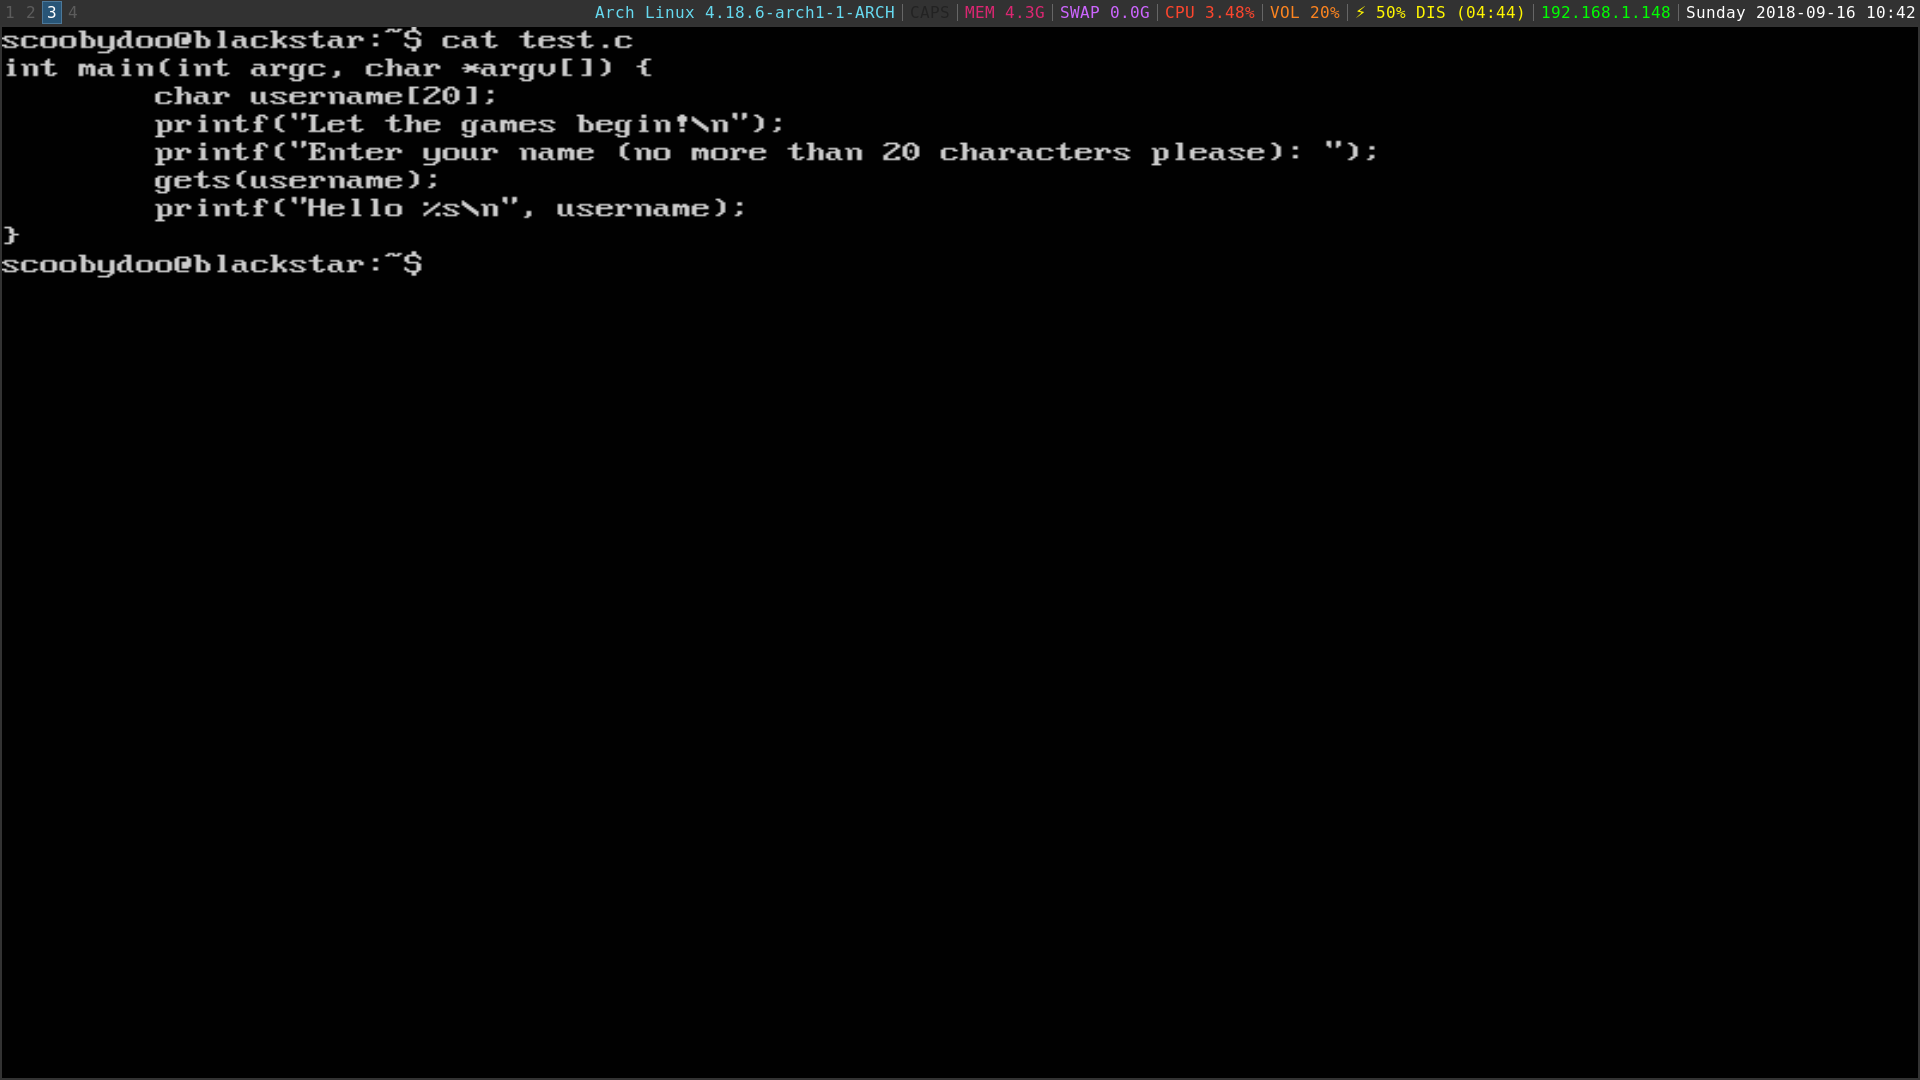
\includegraphics[width=15cm, height=10cm]{test_code.png}
\caption{Poorly written vulnerable C test program}
\end{figure}
\begin{figure}[H]
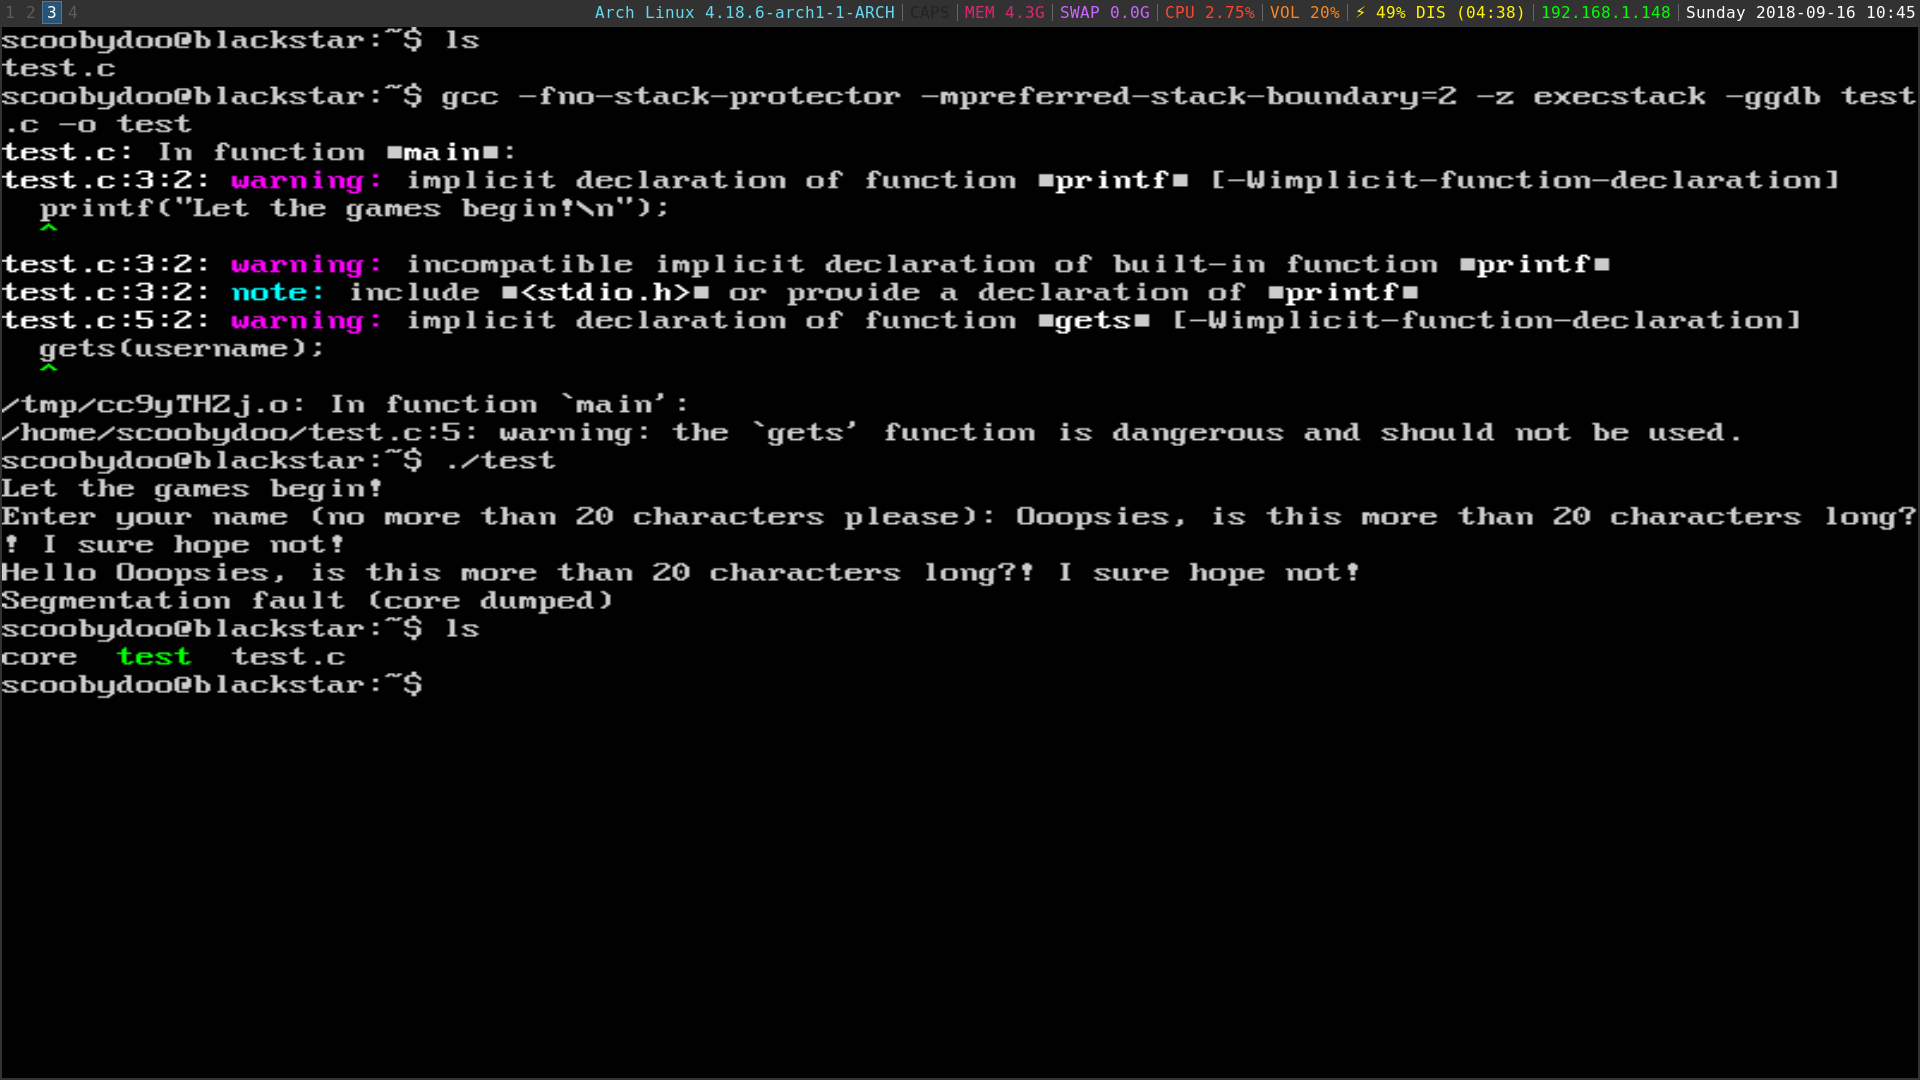
\includegraphics[width=15cm, height=10cm]{compiled_code.png}
\caption{Demonstration of compiling and running the test program}
\end{figure}

\newpage
\section{Raspberry Pi}\label{pi}
\subsection{Installing Raspbian}
First you should get a Raspbian image from \href{https://www.raspberrypi.org/downloads/raspbian/}{here}, I used the Raspbian Stretch Light image as we will not be needing a GUI. You can use dd to move the .img file onto your microSD card:
\begin{verbatim}
sudo dd if=2018-06-27-raspbian-stretch-lite.img of=/dev/sdc bs=4M status=progress
\end{verbatim}
\subsection{Connecting to the Pi using UART}
This may not be directly related to the course but being able to talk to things via serial communication can sometimes be really helpful. UART is a serial protocol that many devices use, manufacturers sometimes use these for debugging their hardware and even leave them open! For example, some routers have serial pins that you can connect to and actually access the operating system it is running directly. In our case, if enabled, we can interact via our raspberry pi through its UART pins. To enable uart, before booting into our pi we can mount the microSD and add a line to its boot options:
\begin{verbatim}
sudo mount /dev/sdc1 /mnt
cd /mnt
echo "enable_uart=1" >> config.txt
cd && sudo umount /mnt
\end{verbatim}
\begin{figure}[H]
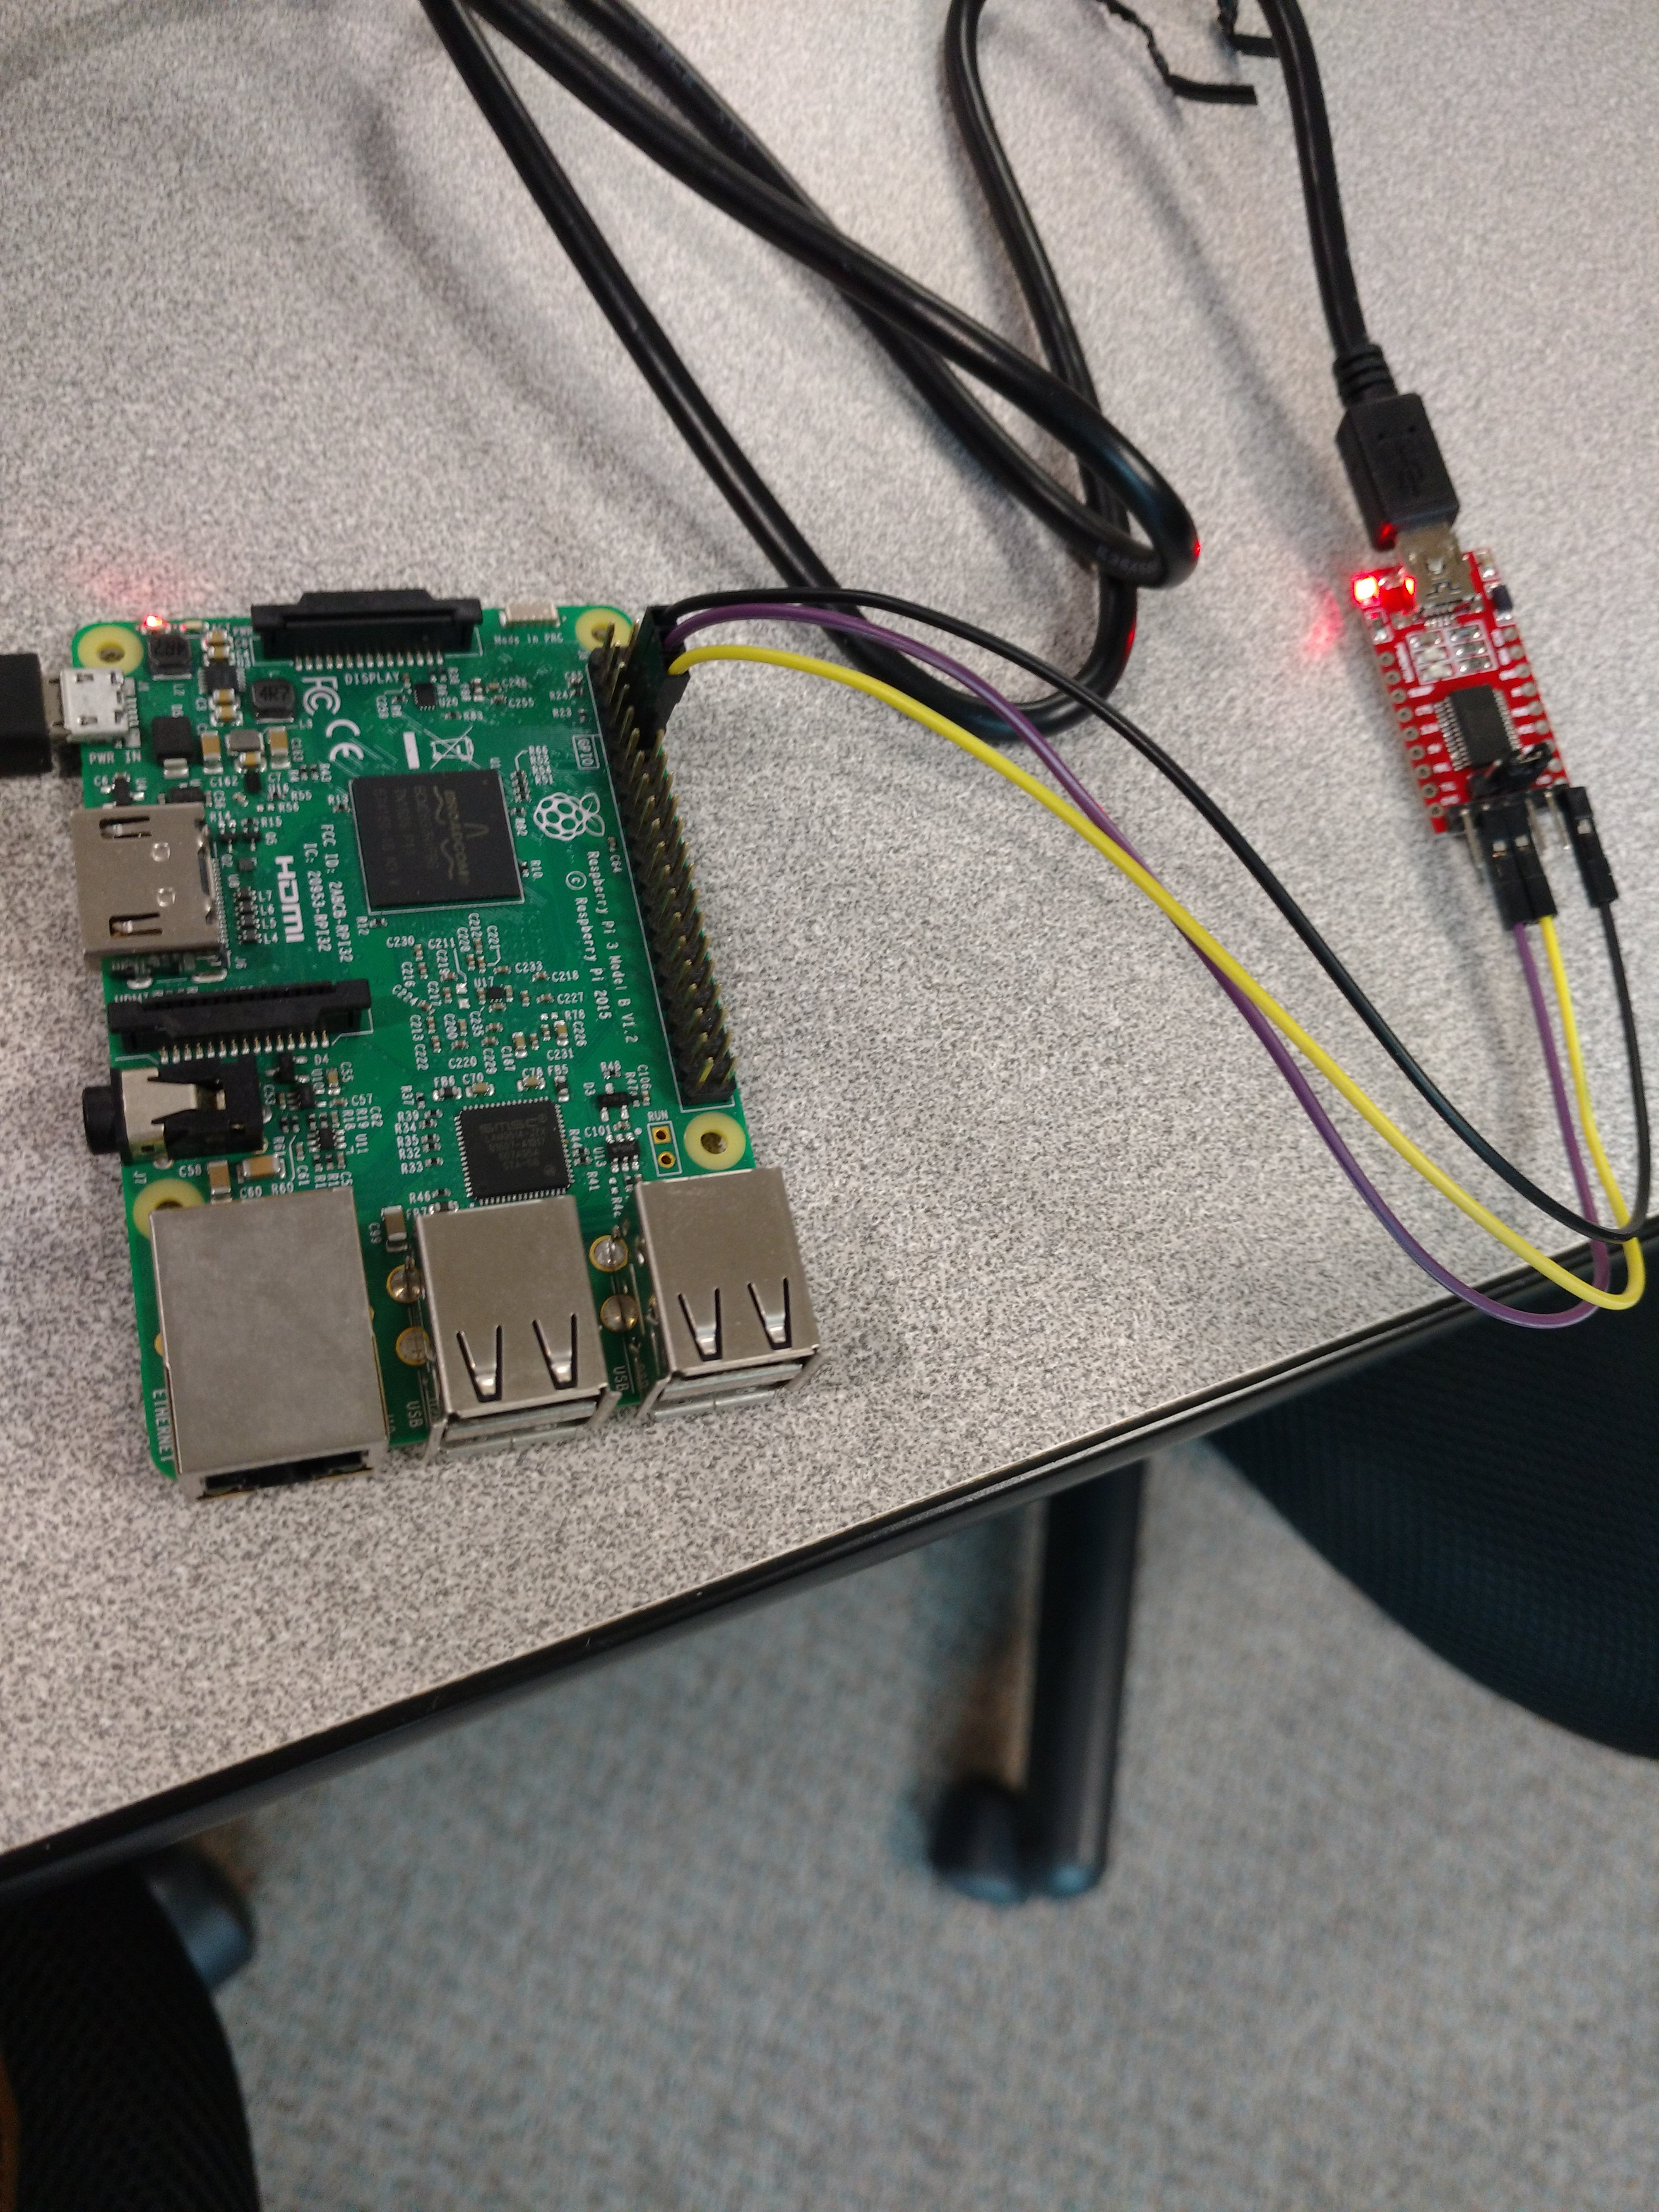
\includegraphics[width=17cm, height=11cm]{pi_uart.png}
\caption{Using a serial-to-usb adapter to connect to our Raspberry Pi}
\end{figure}
Now that the UART is enabled, we can use a \href{https://www.sparkfun.com/products/13830}{serial-to-usb adaptor} like the one connected as shown above and GNU Screen to connect to it.
\begin{verbatim}
sudo screen /dev/ttyUSB0 115200,cs8,-parenb,-cstopb,-hupcl
\end{verbatim}
There we go, we should now have a TTY on our pi where we can run any command just like a regular terminal, no HDMI or internet required!

\subsection{Making the Pi exploitable}
The Raspbian image has Linux kernel version 4.14.50 which means it will have ASLR, luckily the steps are the exact same as above. The version of GCC is 6.3.0 which means we have to specify options to disable some security features and enable debugging, luckily this process is also the same as described above. Thus, if you create the file to disable ASLR and use the GCC options shown above, we will have a sufficiently vulnerable pi to start exploiting!

\section{Conclusions}\label{conclusions}
We now have two environments, one for x86 exploits and another for ARM exploits. We have disabled ASLR and know what arguments to pass to GCC so we can reliably test our exploits. Several security features may have been missed, but the major ones have been covered, if there are other features that stop us we can learn about them and how to deal with them along the way.

\end{document}
